
\chapter[Depth Diversification]{Tiebreaking by Depth Diversification for \astar Search}

\label{chap:tiebreaking}

As shown in the previous section, the search spaces of Zerocost domains have many 0-cost edges,
resulting in a large final plateau ($\plateau{f^*,0}$). In a final plateau,
all nodes have $h=0$, so $h$-based tie-breaking cannot provide
useful guidance toward a goal. Thus, we need a new metric for discriminating among nodes
in the plateau so that the search algorithm can make progress in the plateau.

We define the \emph{depth} of a node as an 
integer representing the distance (number of steps) from the
\emph{entrance} of the plateau.  An \emph{entrance} of the plateau is
the first node which encountered the plateau along the path from the
initial node. These notions are depicted in
\refig{fig:plateau-depiction} (subfigure 1). 

\begin{figure}[htbp]
  \centering
  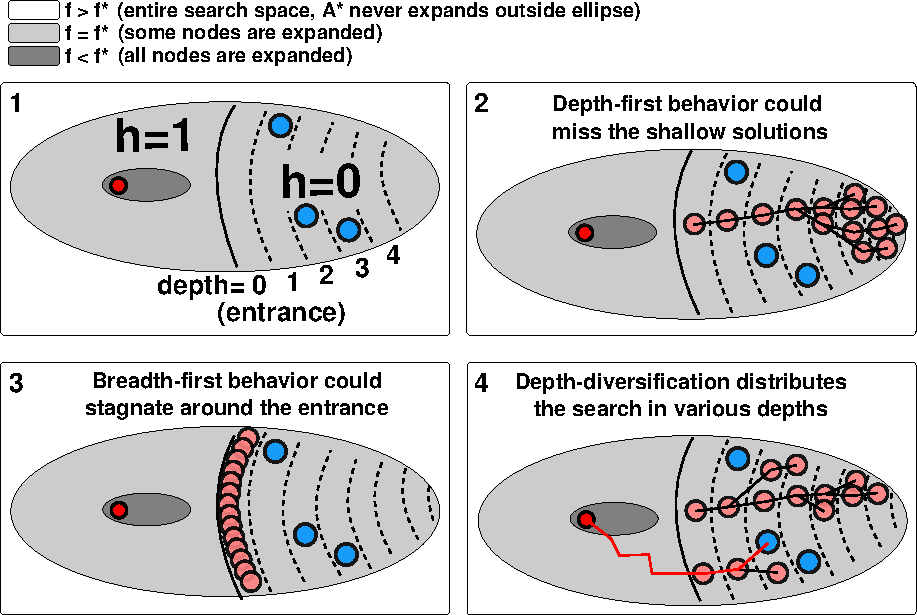
\includegraphics[width=\textwidth]{img/astar/plateau-2.pdf}
 \caption{(\textbf{Subfigure 1}) The nodes in a plateau are divided into several layers, and each layer has a corresponding depth. Since all nodes have $f=f^*$, depth does not affect optimality, so all
goals in the final plateau are cost-optimal, regardless of whether they are in shallow/deep regions.
 (\textbf{Subfigure 2}) \lifo tie-breaking strategy results in depth-first behavior in a
 plateau, which could miss solutions if they are concentrated near the entrance.
 (\textbf{Subfigure 3}) \fifo tie-breaking strategy results in  breadth-first behavior in a
 plateau, which could fail to reach solutions in deeper layers within the time limit.
 (\textbf{Subfigure 4}) Depth-based diversification allows \astar to search the plateau space
 in a less biased manner. This balances exploration and exploitation, avoiding the problems with both \lifo (depth-first) and \fifo (breadth-first) behavior.
 }
 \label{fig:plateau-depiction}
\end{figure}

The depth $d(n)$ of a node $n$ is 0 when $n$ and
the parent node $m$ are in the different plateaus,
and $d(n)=d(m)+1$ when they are on the same plateau.
As defined in \refchap{chap:background}, if two nodes are  on the same plateau, 
they share the same key values for the sorting strategy.
For example, when the strategy is $[f,h,*]$,
 % and $n$ and $m$ are on the same plateau,
it means $\plateau{f(n),h(n)}=\plateau{f(m),h(m)}$, therefore
$f(n) = f(m) \land h(n) = h(m)$.

The traditional \lifo and \fifo tie-breaking strategies
search each plateau in decreasing and increasing order of the depth, respectively.
Assume we are using $[f,h,*]$ sorting strategy.
The \lifo strategy always selects the most recently generated node
within $\plateau{f,h}$, and the behavior in the plateau is equivalent to depth-first search.
Thus, \lifo always selects a node in the largest depth,
as depicted in \refig{fig:plateau-depiction} (subfigure 2).
Similarly, the behavior of \fifo strategy 
in a plateau is equivalent to breadth-first search. Thus \fifo 
always selects the nodes with the least depth (subfigure 3).
Note that  $[f,h,\lifo]$ is equivalent to $[f,h,-d,\lifo]$ and
$[f,h,\fifo]$ is equivalent to $[f,h,d,\fifo]$.

The problem with these traditional strategies is that we have no knowledge
regarding whether the goals are located close to or far from the entrance. Recall
that since $f=f^*$, all goal nodes in the final plateau are optimal with respect to solution cost
regardless of the depth.
%: A goal node in a shallower region or a deeper region both yields a cost-optimal solution. 
However, until we find a
solution, we do not know how the goals are distributed among various
depths. In some problem instances the goals can be concentrated around
the entrance, while in other problem instances the goals can be
concentrated at some large depth. % $k$.  k never used below?

In the former case, \fifo
should perform well because its breadth-first behavior naturally
focuses the search around the entrance, favoring the smaller depths.
However, in the latter case, exhaustively searching
the shallower depths can result in not finding any solutions within
the time limit because \fifo may never reach the depth where the goals
exist.  On the other hand, \lifo behaves in a depth-fist manner, so it
may reach solutions at deeper depths quickly, but risks missing
solutions at shallower depths.  Thus, both \fifo and \lifo tie-breaking
are prone to failures due to pathological cases.

\section{Depth-Based Tie-Breaking for A*}

In order to avoid focusing the search at the wrong depths (too shallow/deep), 
the safest policy seems to be to simply \emph{diversify} the depths which are being searched,
in order to avoid any depth-based biases which could lead to pathological behavior.
In our proposed \emph{depth diversification} strategy, the nodes are inserted into buckets
associated with depths, and upon expansion, search effort is distributed in a more balanced manner
among various depths (\refsec{sec:theoretical-characteristics} defines ``more balanced''  more precisely).
Nodes are not  ``sorted''
according to increasing or decreasing order of depth -- instead, we try to 
``diversify'' the node expansion within the plateau.
We denote this depth diversification criterion as $\depth$. 
For example, $[f,h,\depth]$ first breaks ties according to $h$ values,
then uses the $\depth$ criterion to break ties in $\plateau{f,h}$.
%We denote such a diversification family of
%tie-breaking strategies by enclosing it in brackets such as $[f,h,\depth]$.

\begin{algorithm}
 \textbf{Initialization of Instance Variables:}
\begin{algorithmic}
 \STATE Counter $d_c\leftarrow 0$, Buckets $B=\braces{B_0, B_1,\ \ldots}$, $\forall d; B_d=\emptyset$ (instantiated on-demand)
\end{algorithmic}
 \textbf{Method} $\textbf{push}(\text{node}\ n,\text{selector})$:
\begin{algorithmic}
 \STATE Instantiate $B_{d(n)}$ if it does not exist
 \STATE $\text{push}(n, B_{d(n)})$
\end{algorithmic}
 \textbf{Method} $\textbf{pop}(\text{selector})$:
\begin{algorithmic}[1]
 \LOOP
 \STATE $d_c\leftarrow d_c-1$
 \STATE $d_c\leftarrow \bars{B}-1$ \textbf{if} $d_c<0$
 \IF{$B_{d_c} \not= \emptyset$}
 \RETURN $\text{pop}(B_{d_c})$ --- Note: Actual ``pop'' method is subject to default tiebreaking.
 \ENDIF
 \ENDLOOP
\end{algorithmic}
\caption{Class Definition of Depth-Diversified Node Selector}
\label{alg:depth}
\end{algorithm}

In order to diversify the expansion among depths, we simply
iterate over the depth buckets (\refalgo{alg:depth}).
This iteration is managed by a Depth-Diversified Node Selector instance associated with each plateau (e.g. each of $\plateau{1,0}, \plateau{2,0}, \plateau{2,1}\ldots$).
In order to select a single node from the OPEN list for expansion,
we first select the plateau with the smallest key value, such as $\plateau{f=5,h=1}$, as usual.
This plateau is now represented by a selector instance, and
we call $\text{pop}(\text{selector})$ method on this instance in order to obtain a node.
Each instance holds
an index $d_c$,
the current depth (bucket index) selected in the last expansion,
initialized to 0.
On each call to $\text{pop}(\text{selector})$,
% At each expansion, 
the counter is decremented ($d_c\leftarrow d_c-1$) and
a node is further popped from $d_c$-th bucket, which can be a \lifo, \fifo or \ro queue.
When $d_c$ reaches below 0, then $d_c$
is reset to the current largest depth in the plateau.

In an earlier, conference paper, we used a non-deterministic,
randomized implementation of this idea \cite{Asai2016}, which does not have this counter and pops a node from a randomly selected bucket ($B_{\texttt{random}()}$), but we use a deterministic
implementation here because it facilitates the theoretical analysis below in \refsec{sec:theoretical-characteristics}.
%It also eliminates the possibility of results being influenced by random seeds. %  this eliminates randomness within the deph diversification, but there can be other random factors, e.g., ro default tiebreaking, so "eliminates" is too strong.

Depth-based diversification is significantly different from the \ro strategy which simply selects a random node from the OPEN list.
The uniform sampling behavior of  \ro behaves very similar to \fifo, and is insufficient to achieve the level of diversity provided by our depth diversification tie-breaking,
which is also already evidenced by the performance similarity between \fifo and \ro-based tiebreaking strategies (\reftbl{tbl:summary-std}).
This is because at any given point in the search, more nodes will tend to have shallower depths than deeper depths, and a uniform, random selection will, therefore, be biased to select a node with shallow depths.
For example, imagine we have 100 nodes at depth $d=1$ and a single node at depth $d=2$.
Since \ro does not consider the depth, the chance of expanding $d=2$ is only $1/101$.
This probability does not improve until a sufficient number of expansions decreases the number of nodes in $d=1$.
In contrast, our depth diversification policy expands nodes at $d=1$ and $d=2$ with equal probability.


% We later show that
% \fifo and \lifo strategies are incomplete when the size of the plateau
% region is inifinite, while our \id is probabilistically complete.

% \subsection{When Does Depth-Based Tie-Breaking Affect Node Expansion Order?}
% \label{sec:depth-and-nonzero-cost}

% ``no effect'' is ambiguous, reviewers may complain that we are trying to claim there is no overhead, including the low level overhead. Thus I reworded from ``no effect'' to ``does not affect the order of expansion''.
Depth-based tie-breaking does not affect the order of node expansion when there are no remaining ties after the
higher priority tie-breaking criteria, in which case all nodes have depth 0.
\todo*{mentioning ``keys'' seems unnecessarily complicated, so remove it}
More formally:

%\begin{theo}
%  When all edge costs are positive,    
% the depth of the nodes expanded by \astar $[f,h,\depth,*]$ is always 0
% and depth diversification does not affect the expansion ordering.
%\end{theo}
%\begin{proof}
%Let a node $n$ be a child of a node $m$.
%Regardless whether the parent $m$ of the node $n$ is newly assigned, updated, or the old parent is kept,
%the invariant $g(n)=g(m)+\mit{cost}(m,n) > g(m)$ holds due to the positive edge cost, and therefore $f(n)-h(n) > f(m)-h(m)$.
%This means that either $f(n)\not=f(m)$ or $h(n)\not=h(m)$ and the depths of nodes are always 0.
%\end{proof}

% expansion ordering of \astar on the plateau is not affected by depth diversification 

\begin{lemma} 
 \label{lemma:depth0}
  If all edge costs are positive, then
  $d(n) = 0$ for every node $n$ expanded by \astar $[f,h,\depth,*]$.
\end{lemma}
\begin{proof}
Let $n$ be a child of a node $m$.
Regardless whether the parent $m$ of the node $n$ is newly assigned, updated, or the old parent is kept in line 10 of \refalgo{alg:ocl},
the invariant $g(n)=g(m)+\mit{cost}(m,n) > g(m)$ holds
%due to the positive edge cost,
because $\mit{cost}(m,n)>0$,
and therefore $f(n)-h(n) > f(m)-h(m)$.
This means that either $f(n)\not=f(m)$ or $h(n)\not=h(m)$, so $d(n) = 0$.
\end{proof}


\begin{theo}
  If all edge costs are positive, then \astar $[f,h,\depth,*]$ expands nodes in the same order as  \astar $[f,h,*]$ (where ``$*$'' is any criterion).
\end{theo}
\begin{proof}
  By Lemma \ref{lemma:depth0}, all nodes expanded by \astar $[f,h,\depth,*]$ have depth 0, and all nodes are in the same depth bucket in \refalgo{alg:depth}, so \astar $[f,h,\depth,*]$ expands nodes in the same order as \astar $[f,h,*]$ regardless of the criterion $*$.
\end{proof}


\subsection{Tie-Breaking within Depth Buckets}

Depth diversification cannot be a default tie-breaking by itself.
Consider a tie-breaking strategy such as $[f,h,\depth]$ which applies a depth-diversification tie-breaking.
After the $\depth$ criterion is applied, 
there may be multiple nodes within the same depth bucket, so a
default tie-breaking criterion is still necessary to break ties among them.
Thus, we should, for example, apply one of \lifo, \fifo or \ro (random order) criteria
after the $\depth$ criterion.

There are two concerns about this default tie-breaking criteria.
First, the default tie-breaking behavior is still susceptible to 
 accidental biases, e.g., names/orders of action schema in the PDDL domain definition \cite{vallati2015effective}.
Second, in addition to accidental biases, there may be some nontrivial biases that require 
sophisticated algorithms to be removed.

Recent work  showed that the performance of a satisficing
planner can be significantly affected by the order in which actions appear in a PDDL file \cite{vallati2015effective}.
However, the conference version of this paper \cite{Asai2016} showed that
the effect of such an accidental bias is not statistically significant in cost-optimal search,
by comparing the performance on
several sets of randomly ``mangled'' domains whose action names are replaced with random strings.
Moreover, the \ro default tie-breaking should be unaffected by such an accidental bias.
Thus, we believe it is safe to claim that the experimental results in this paper are not a product of such accidental biases.

% ``breadth direction'' example was not well defined, replaced with vague discussion of symmetry (combined with the next par); also removing ``non-trivial'' because trivial/nontrivial is not obvious and undefined.
In addition to accidental biases, there may be other nontrivial biases such as some form of symmetry among states which can be removed using some tie-breaking criterion $X$.
Such a criterion can be applied after the depth criterion but before the default criterion,
resulting in a sorting strategy $[f,h,\depth,X,\fifo]$. 
Candidates for $X$ may be related to pruning techniques such as Symmetry Breaking \cite{Fox1998,pochter2011exploiting,domshlak2013symmetry} or
Partial Order Reduction \cite{hall2013faster,wehrle2013relative}.
While these are usually described as ``pruning techniques'',
they can also be interpreted as strong bias removal mechanisms because
they seek to prune redundant nodes, and 
redundancy causes a biased search effort. For example, imagine we have a
set of nodes $S=\{a_1, a_2, a_3, a_4, b, c, d\}$ where
$A=\{a_1, a_2, a_3, a_4\}$ are ``redundant'' according to some measure (e.g. by Symmetry,
Partial-Order). 
If a search algorithm expands $S$ by random selection, it favors the
group $A$ by giving 4 times larger chance of expansion than each of $b$,
$c$ or $d$.
Despite this similarity, search diversification is weaker than pruning methods because diversification can only \emph{delay} the expansion of nodes sharing the similar attributes (such as depth), not \emph{prune} the nodes.
%Developing a diversification method addressing biases similar to those by pruning techniques is an avenue for future work.


\subsection{Theoretical Characteristics of the Depth Distribution}
\label{sec:theoretical-characteristics}

We give further insight into the search behavior of our implementation of depth-based diversification.
In depth-based diversification, although it is possible to select from a randomly selected depth bucket, as was done in an earlier conference paper \cite{Asai2016},
the implementation used in this paper performs a deterministic, round-robin sampling from the available depth buckets as described in \refalgo{alg:depth}.
%iterates from the largest depth to 0.
% 
%We are particularly interested in how the expansions happen among the
%various depths in the plateau region.
We are particularly interested in how the nodes selected for expansion are distributed 
among the various depths in a plateau region.
Assume that a search algorithm is searching a plateau region $P$.
The precise definition of $P$ depends on the higher-level sorting strategy e.g. $[f,h,\depth]$ or $[f,\depth]$.
% 
Using a simplified model where this $P$ forms a forest (a set of disjoint trees),
we can analyze the number of expansions in a particular depth
can be represented by a simple formula. 
% Although the notion of
% probability does not fit well with deterministic \fifo or \lifo
% default tie-breaking, it is still meaningful in the case of \ro (random
% order) default tie-breaking.

%% danger!!
% \begin{theo}[Uniformness of the search]
%  Assume the search space forms a forest of fixed width $w\geq 2$.
%  After enough number of iterations $D$,
%  the chance of expanding each node is unaffected by the depth of the
%  node, if the depth $d$ is small relative to $D$.
% \end{theo}

% I no longer claim the distribution is uniform.

% As a preparation, we first show that the number of expansion happened to each depth decreases
% linearly with the depth.

% 
\todo*{Introduced the forest assumption in the beginning.}
In the discussion below, 
we first assume that $P$ forms a forest of a fixed branching factor
$w\geq 2$ (\emph{forest assumption}), rather than a graph with an indefinite number of successor nodes.
In the later experiments, we show this is a fairly accurate model.
We also assume that no depth bucket is exhausted due to the expansion (\emph{no-exhaustion assumption}). This implies that there are a sufficiently large number of nodes in depth $d=0$ so that depth 0 is not exhausted, which may cause \fifo default tiebreaking to fail due to the heavy bias to the shallow depth.
We provide a condition for this assumption to hold within this section.
% Finally, we assume that the sorting strategy performs a \ro default tie-breaking
% after the depth-based diversification is applied.
An example of running depth diversification with $w=3$ is depicted in \refig{fig:depth-distribution-analysis}.

\begin{figure}[htbp]
  \centering
  % 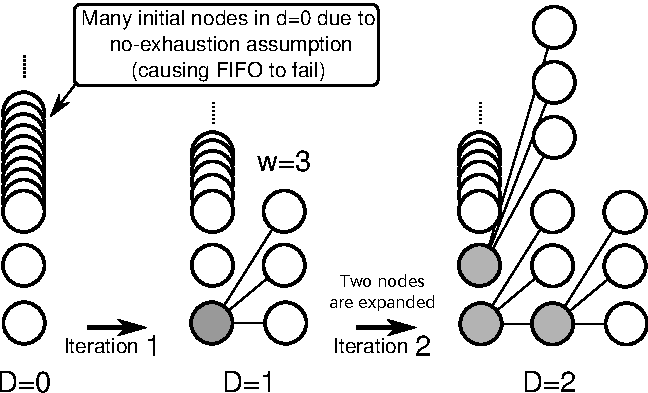
\includegraphics{img/depth-distribution-analysis.png}
  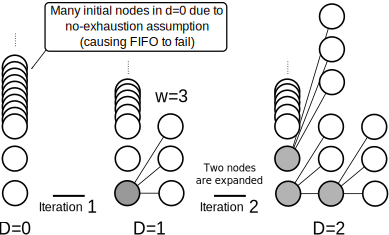
\includegraphics{img/depth-distribution-analysis/depth.pdf}
 \label{fig:depth-distribution-analysis}
 \caption{Depth Diversification applied to a plateau 
with forest assumption and no-exhaustion assumption.}
\end{figure}

Let $D\geq 0$ be the current largest depth of the nodes found in $P$ so far.
This is equal to $\bars{B}-1$ in \refalgo{alg:depth},
the size of the buckets in Depth-Diversified Node Selector instance.
An expansion of a node at depth $D$ results in $w$ more nodes with depth $D+1$ on the same plateau $P$.
These children are all newly generated because by the forest assumption, each child has a single incoming edge.
Since the expansion is
diversified by a sequence of iterations from the current largest depth to 0, when the current
largest depth of the plateau is $D$, the number of iteration executed so far is also $D$ because
at the beginning of each iteration the largest depth is increased by 1.
% Under the forest assumption, each expansion of depth $d$ results in $w$ new nodes in depth $d+1$. 
Therefore, at the end of the $D$'th iteration,
each depth $d$ has been expanded exactly $D-d$ times, with $D(D-1)$ expansions in total.
In \refig{fig:depth-distribution-analysis},
after iteration 2, depth $d=0$ is expanded twice and depth $d=1$ is expanded once.

It also means that a sufficient condition for \emph{no-exhaustion assumption} to hold until the end of the $D$'th
iteration is that the initial number of nodes in depth 0 is at least $D$.  If there are at least $D$ nodes in depth
0, depth 0 is trivially never exhausted until the $D$'th iteration. Also, no depth buckets in depth $d>0$ will be exhausted 
because each bucket has $w(D-d+1)$ generated nodes in total (i.e. OPEN+CLOSED) while the expansion has
happened only $D-d$ times.
The number of nodes in each bucket ($w(D-d+1)$) follows from the fact that  depth $d-1$ is expanded $D-(d-1)$ times in the preceding $D$ iterations.
Since $w\geq 2$, $w(D-d+1)\geq 2(D-d)+2>D-d$.
% For simplicity, let us also assume that the depth 0 initially have exactly $D$ nodes and
% no nodes will be added to depth 0 during the search.
% Also let $N=w(D-d+1)$ for readability.

If there are no solutions, every depth-selection criterion, including least depth selection (\fifo) or largest depth selection (\lifo), expands the same set of nodes and results in the same distribution as depth diversification.
For example, if the number of nodes in depth 0 is $D$, each $d$ is expanded $Dw^d$ times.
However, their online characteristics are different.
Under our assumptions, the $D-d$ distribution of depth diversification is an invariant which holds at any point in the search until the solution is found.
In contrast, in \fifo, all nodes with $d<D-1$ are expanded, depth $d=D-1$ can take an arbitrary number of expansions $e \in [0, Dw^{D-1}]$ and $d\geq D$ are not expanded at all.
In \lifo, for some $k\in [0,D_\mit{max}]$ (assuming the forest has a finite maximum depth $D_\mit{max}$), there can be a situation where all depths $d \in [0,k]$ get only 1 expansion each
while all nodes in depths $d \in [k+1,D_\mit{max}]$ are expanded. In this case, the number of expansions in $d \in [k,D_\mit{max}]$ is exponential to $D_\mit{max}-k$ ($\sum_{i=k}^{i=D\mit{max}}w^{i-k}=\frac{1-w^{D\mit{max}-k+1}}{1-w}$) while the number of expansions in $d \in [0,k-1]$ is linear to $k$ (i.e. $k-1$). Such an imbalance during the search causes the pathological behavior mentioned above.


\begin{figure}[htbp]
  \centering
  % 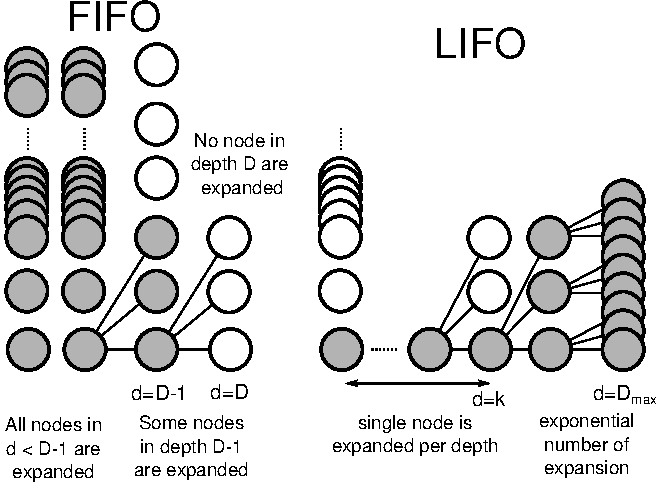
\includegraphics{img/depth-distribution-analysis-fifolifo.png}
  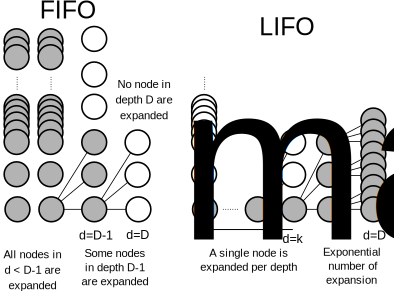
\includegraphics{img/depth-distribution-analysis/fifolifo.pdf}
 \label{fig:depth-distribution-analysis-fifolifo}
 \caption{FIFO and LIFO applied to a plateau
 with forest assumption and no-exhaustion assumption.}
\end{figure}


\todo*{maybe \lifo and \fifo should be analyzed wrto this forest model and compared directly to each other as well as
$\depth$?}
\todo*{less priority -- lets add it when required by the reviewers. unused texts are in unused/lifo-fifo-distribution.tex}

